\Titelbanner{2}{Lineare Gleichungssysteme}

\textbf{Aufgabe 1: } \emph{Zwei lineare Gleichungen mit zwei Unbekannten}
\begin{enumerate}[label=(\alph*)]
    \item $\{(x\,;y)\} = \qty{\qty(\frac{7}{11}\,;\frac{1}{3})}$
    \item $\{(x\,;y)\} = \qty{\qty(\frac{1}{3}\,;\frac{1}{4})}$
    \item $\{(x\,;y)\} = \qty{\qty(-1\,;0)}$
    \item $\{(x\,;y)\} = \qty{\qty(\frac{b}{a}+1\,;\frac{a}{b}-1)}$
    \item $\{(x\,;y)\} = \qty{\qty(\frac{1}{\sqrt{2}}\,;-\frac{1}{\sqrt{2}})}$
    \item $\{(x\,;y)\} = \qty{\qty(a(a+b)\,;b(a-b))}$
    \item $\{(x\,;y)\} = \qty{\qty(\frac{1}{13}\,;\frac{1}{19})}$
\end{enumerate}
\vspace{0.7cm}
%
\textbf{Aufgabe 2: } \emph{Drei Gleichungen mit drei Unbekannten}
\begin{enumerate}[label=(\alph*)]
\item $\{(x\,;y\,;z)\} = \{(1\,;1\,;1)\}$
\item $\{(x\,;y\,;z)\} = \{(1\,;2\,;3)\}$
\item $\{(x\,;y\,;z)\} = \{(a\,;b\,;c)\}$
\item $\{(x\,;y\,;z)\} = \{(2z\,;5z\,;z)\ |\ z\in\mathbb{R}\}$
\end{enumerate}
\vspace{0.7cm}
%
\textbf{Aufgabe 3: } \emph{Parametrisierung von Lösungsmengen}
\begin{enumerate}[label=(\alph*)]
\item $\{(x\,;y)\} = \qty{\qty(\frac{1+7\lambda}{13}\,;\lambda)\ |\ \lambda\in\mathbb{R}}$
\item $\{(x\,;y)\} = \{(6+7n\,;11+13n)\ |\ n\in\mathbb{N}_0\}$
\end{enumerate}
\vspace{0.7cm}

\textbf{Aufgabe 4: } \emph{Gleichungssysteme}
\begin{enumerate}[label=(\alph*)]
\item $\{(x\,;y)\}=\{(2\,;4),(4\,;2)\}$
\item $\{(x\,;y)\}=\{(17\,;6)\}$
\item $\{(x\,;y)\}=\{(-3\,;-3),(-1\,;1)\}$
\end{enumerate}
\vspace{0.7cm}

\textbf{Aufgabe 5: }\emph{Ungleichungssysteme}
\begin{enumerate}[label=(\alph*), labelindent=1em,labelsep=0.5cm]
\item$~$\\[-0.4cm]
\begin{minipage}{0.2\textwidth}
    \begin{alignat*}{3}
        2x-3y&\geq -6\,,\\
        x-2y&< 11\,,\\
        x&>-y-1\,,\\
        x&<5\,,\\
        x&\geq 0\,,\\
        y&\geq 0
    \end{alignat*}
\end{minipage}
\begin{minipage}{0.8\textwidth}
    \centering
        \begin{tikzpicture}
            \begin{axis}[disabledatascaling, axis lines=middle, xlabel={x}, ylabel={y}, height=7.8cm, domain=-2:10, xmin=-3,xmax=11, ymin=-8, ymax=9, axis equal, legend pos= outer north east]
                \addplot[no marks, black, thick, ]{2/3*x+2};
                \addplot[no marks, FSUblau, thick]{0.5*x-11/2};
                \addplot[no marks, Gruen, thick]{-x-1};
                \draw[thick, PAForange, thick] (5,-8)--(5,8)node[right]{$x<5$};
                \fill[FSUblau, fill opacity =0.3] (0,0)--(5,0) --(5,16/3) -- (0,2) -- cycle;
                \legend{$\textstyle y = \frac{2}{3}x+2$, $\textstyle y = \frac{1}{2}x-\frac{11}{2}$, $\textstyle y = -x-1$};
            \end{axis}
        \end{tikzpicture}
\end{minipage}
Offenbar können die zweite und dritte Ungleichung weggelassen werden, ohne dass sich etwas am eingefärbten Gebiet ändert. 

\item Die Ungleichungen beschreiben eine dreiseitige, unendlich ausgedehnte Pyramide, deren Spitze im Koordinatenursprung sitzt und deren Seiten jeweils die $x$-$y$-, $x$-$z$- und $y$-$z$-Ebene halbieren.\\
\begin{center}
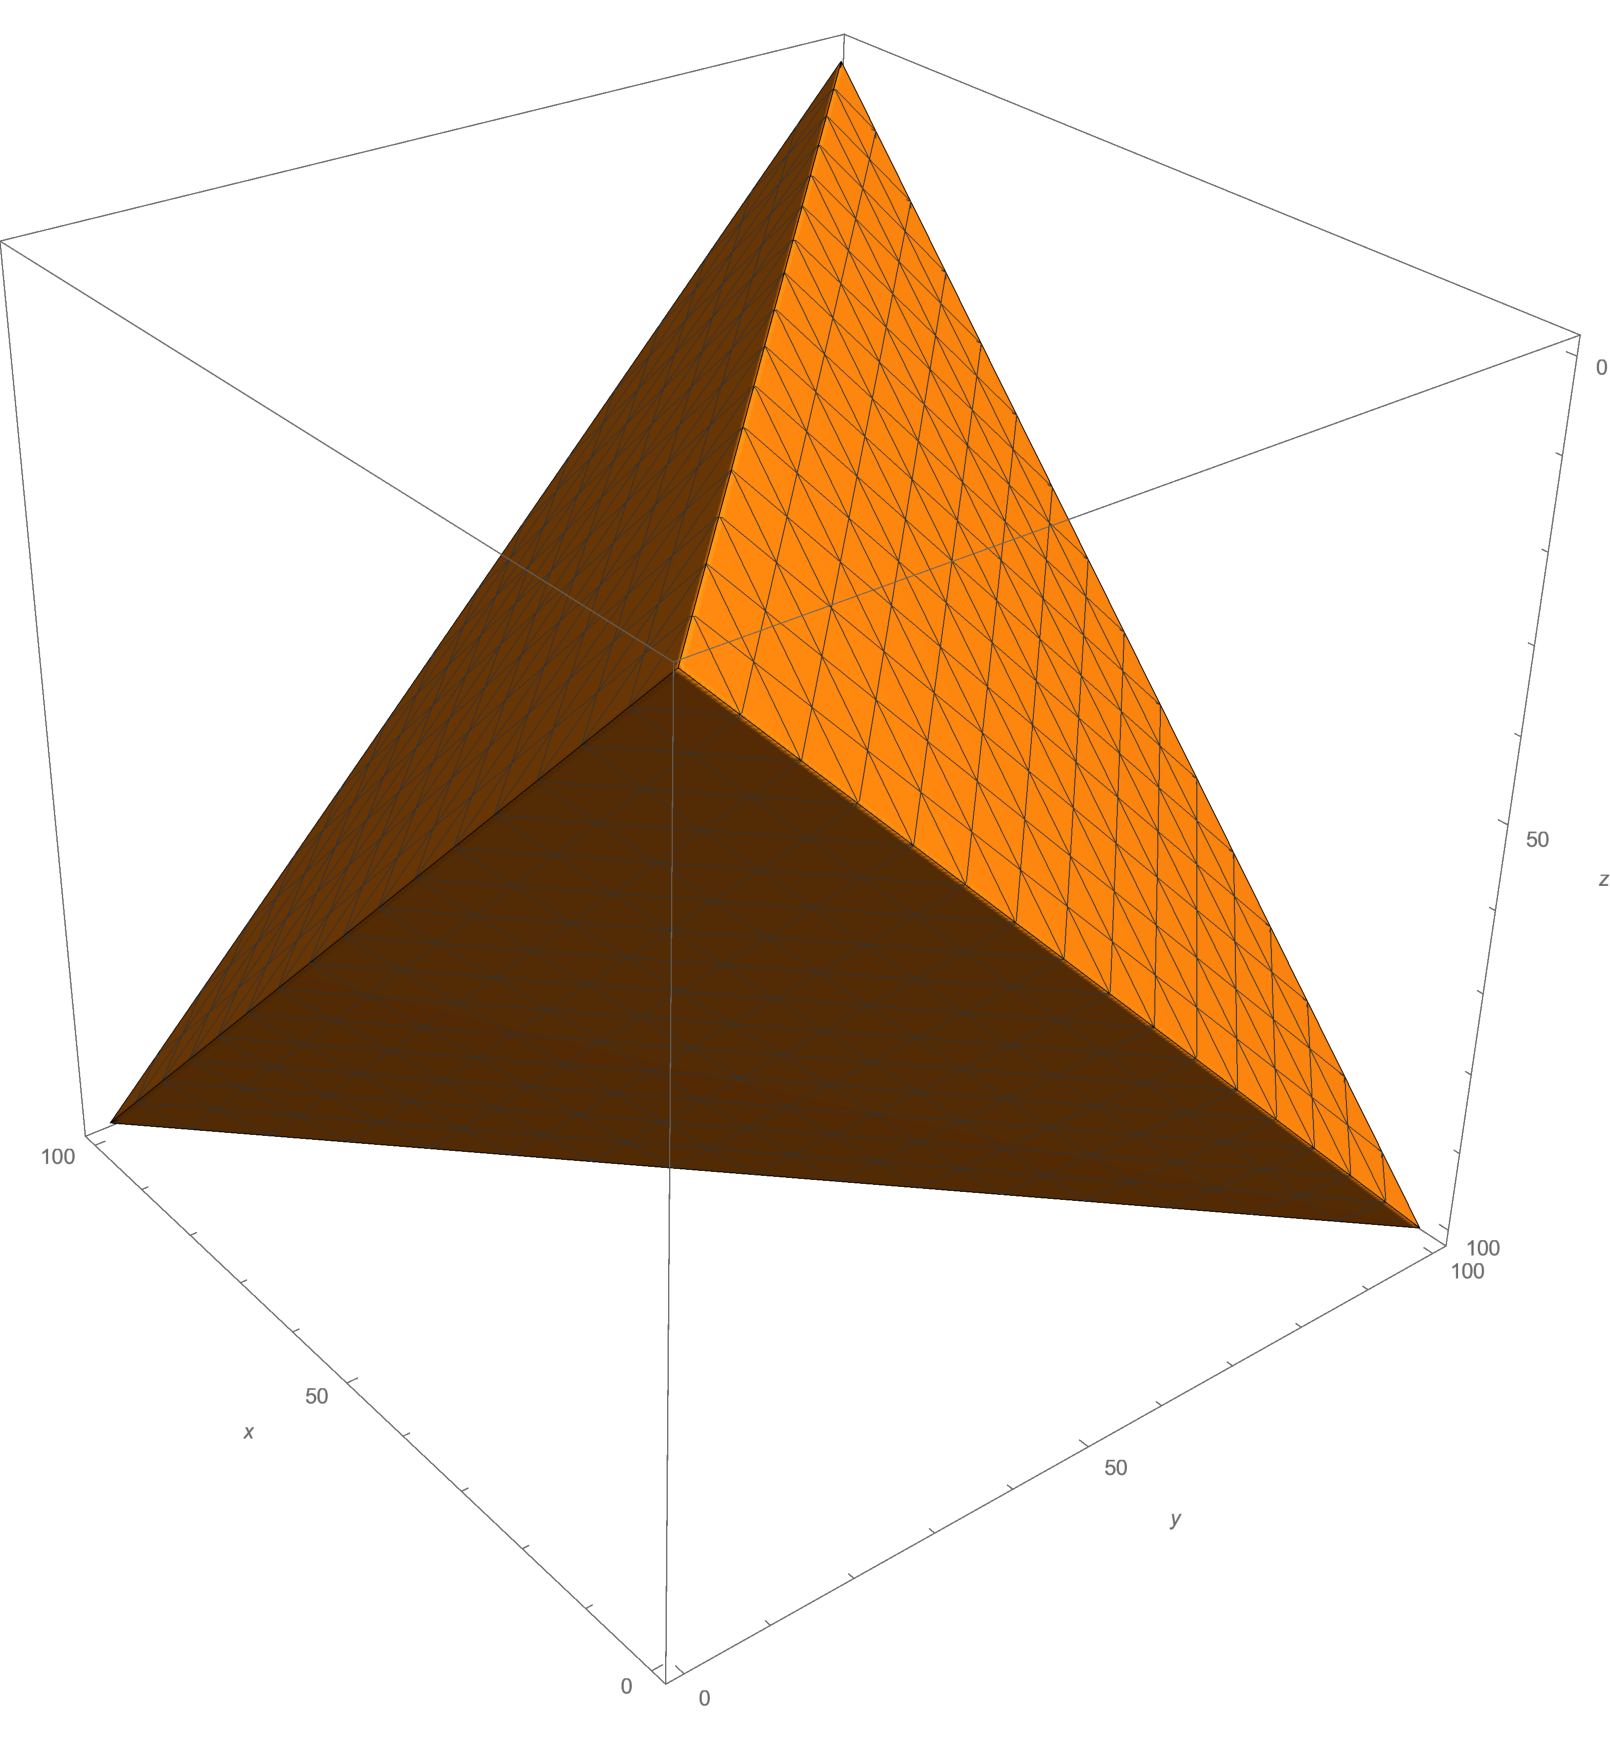
\includegraphics[scale=0.25]{entropy_cone.pdf}
\end{center}

\end{enumerate}